\documentclass[a4paper, 11pt]{article}
\usepackage{comment} % enables the use of multi-line comments (\ifx \fi) 
\usepackage[top = 0.5in, bottom=0.5in]{geometry}
\usepackage{color, listings, graphicx,float, booktabs, tabularx, multirow, amsmath}
\usepackage[colorlinks=true, urlcolor=blue]{hyperref}

\definecolor{codegreen}{rgb}{0,0.6,0}
\definecolor{codegray}{rgb}{0.5,0.5,0.5}
\definecolor{codepurple}{rgb}{0.58,0,0.82}
\definecolor{backcolour}{rgb}{0.95,0.95,0.92}
 
\lstdefinestyle{mystyle}{
    backgroundcolor=\color{backcolour},   
    commentstyle=\color{codegreen},
    numberstyle=\tiny\color{codegray},
    stringstyle=\color{codepurple},
    basicstyle=\footnotesize,
    breakatwhitespace=false,         
    breaklines=true,                 
    captionpos=b,                    
    keepspaces=true,                 
    numbers=left,                    
    numbersep=5pt,                  
    showspaces=false,                
    showstringspaces=false,
    showtabs=false,                  
    tabsize=2
}
\lstset{style=mystyle}

\begin{document}
\graphicspath{{./figures/}}
\noindent
\large\textbf{Kyle Salitrik (kps168)} \\
\normalsize STAT 462\\
\large{Homework 3 Report} \hfill 







%%%%%%%%%%%%%%%%%%%%%%%%%%%%%%%%%%%%%%%%%%%%%%%%%%%%%%%%%%%%%%%%%%%%
%%% SECTION: Applied
%%%%%%%%%%%%%%%%%%%%%%%%%%%%%%%%%%%%%%%%%%%%%%%%%%%%%%%%%%%%%%%%%%%%
\section*{Applied Analysis}
\subsection*{Part A}
Same following on the data was performed:
\begin{itemize}
	\item Samples below 2\% and above 40\% body fat were excluded. The minimum was obtained through the chart on the (\href{''https://www.acefitness.org/acefit/healthy-living-article/60/112/what-are-the-guidelines-for-percentage-of-body-fat-loss''}{\underline{ACE}}) website and maximum was set to limit outliers.
	\item The minimum height accepted was cut to be over 50 inches to remove outliers.
	\item The maximum weight was also clipped to be below 300 pounds. Although the outlier may have been legitimate, it could have also been an error.
	\item Observation number 41 was removed as an influential point.
\end{itemize}

\begin{figure}[H]
	\centering
	\caption{Full Model Q-Q Plot}
	\centerline{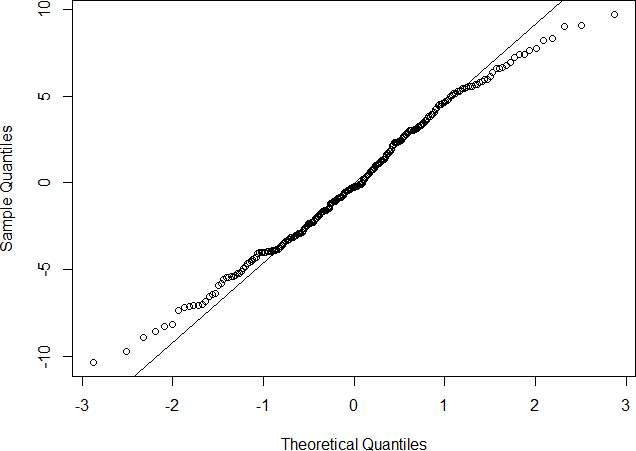
\includegraphics[width=\textwidth]{full_qq_plot.png}}
\end{figure}


%%%%%%%%%%%%%%%%%%%%%%%%%%%%%%%%%%%%%%%%%%%%%%%%%%%%%%%%%%%%%%%%%%%%
%%% SECTION: CODE APPENDIX
%%%%%%%%%%%%%%%%%%%%%%%%%%%%%%%%%%%%%%%%%%%%%%%%%%%%%%%%%%%%%%%%%%%%

%\newpage
%\section*{R Code}
%\lstinputlisting[language=R]{../hw3.r}

\end{document}
